Créer un compte ChromaCase en utilisant Google vous permet d’utiliser votre compte Google pour vous connecter sur ChromaCase, vous évitant ainsi de retenir un nouveau nom d’utilisateur et mot de passe.
\\\\
Pour créer un compte ChromaCase en utilisant votre compte Google, il faut cliquer sur le bouton " for free" en bas de la page d'accueil.

\begin{figure}[H]
	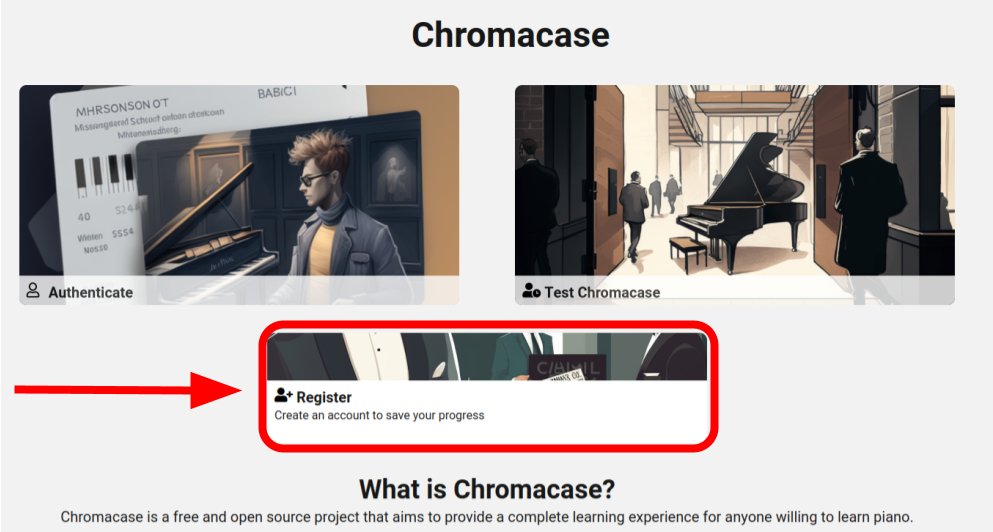
\includegraphics[width=\linewidth]{../\dir/guide/auth/register.png}
	\caption{Créer un compte}
\end{figure}

Cliquez sur le bouton “Continuer avec Google” (Voir Capture \ref{fig:signup-google}). Vous serez redirigé.e vers un formulaire de connexion de Google. Une fois celui-ci rempli et validé, votre compte ChromaCase sera créé, et vous serez redirigé.e vers votre page personnelle.

\begin{figure}[H]
	\begin{center}
		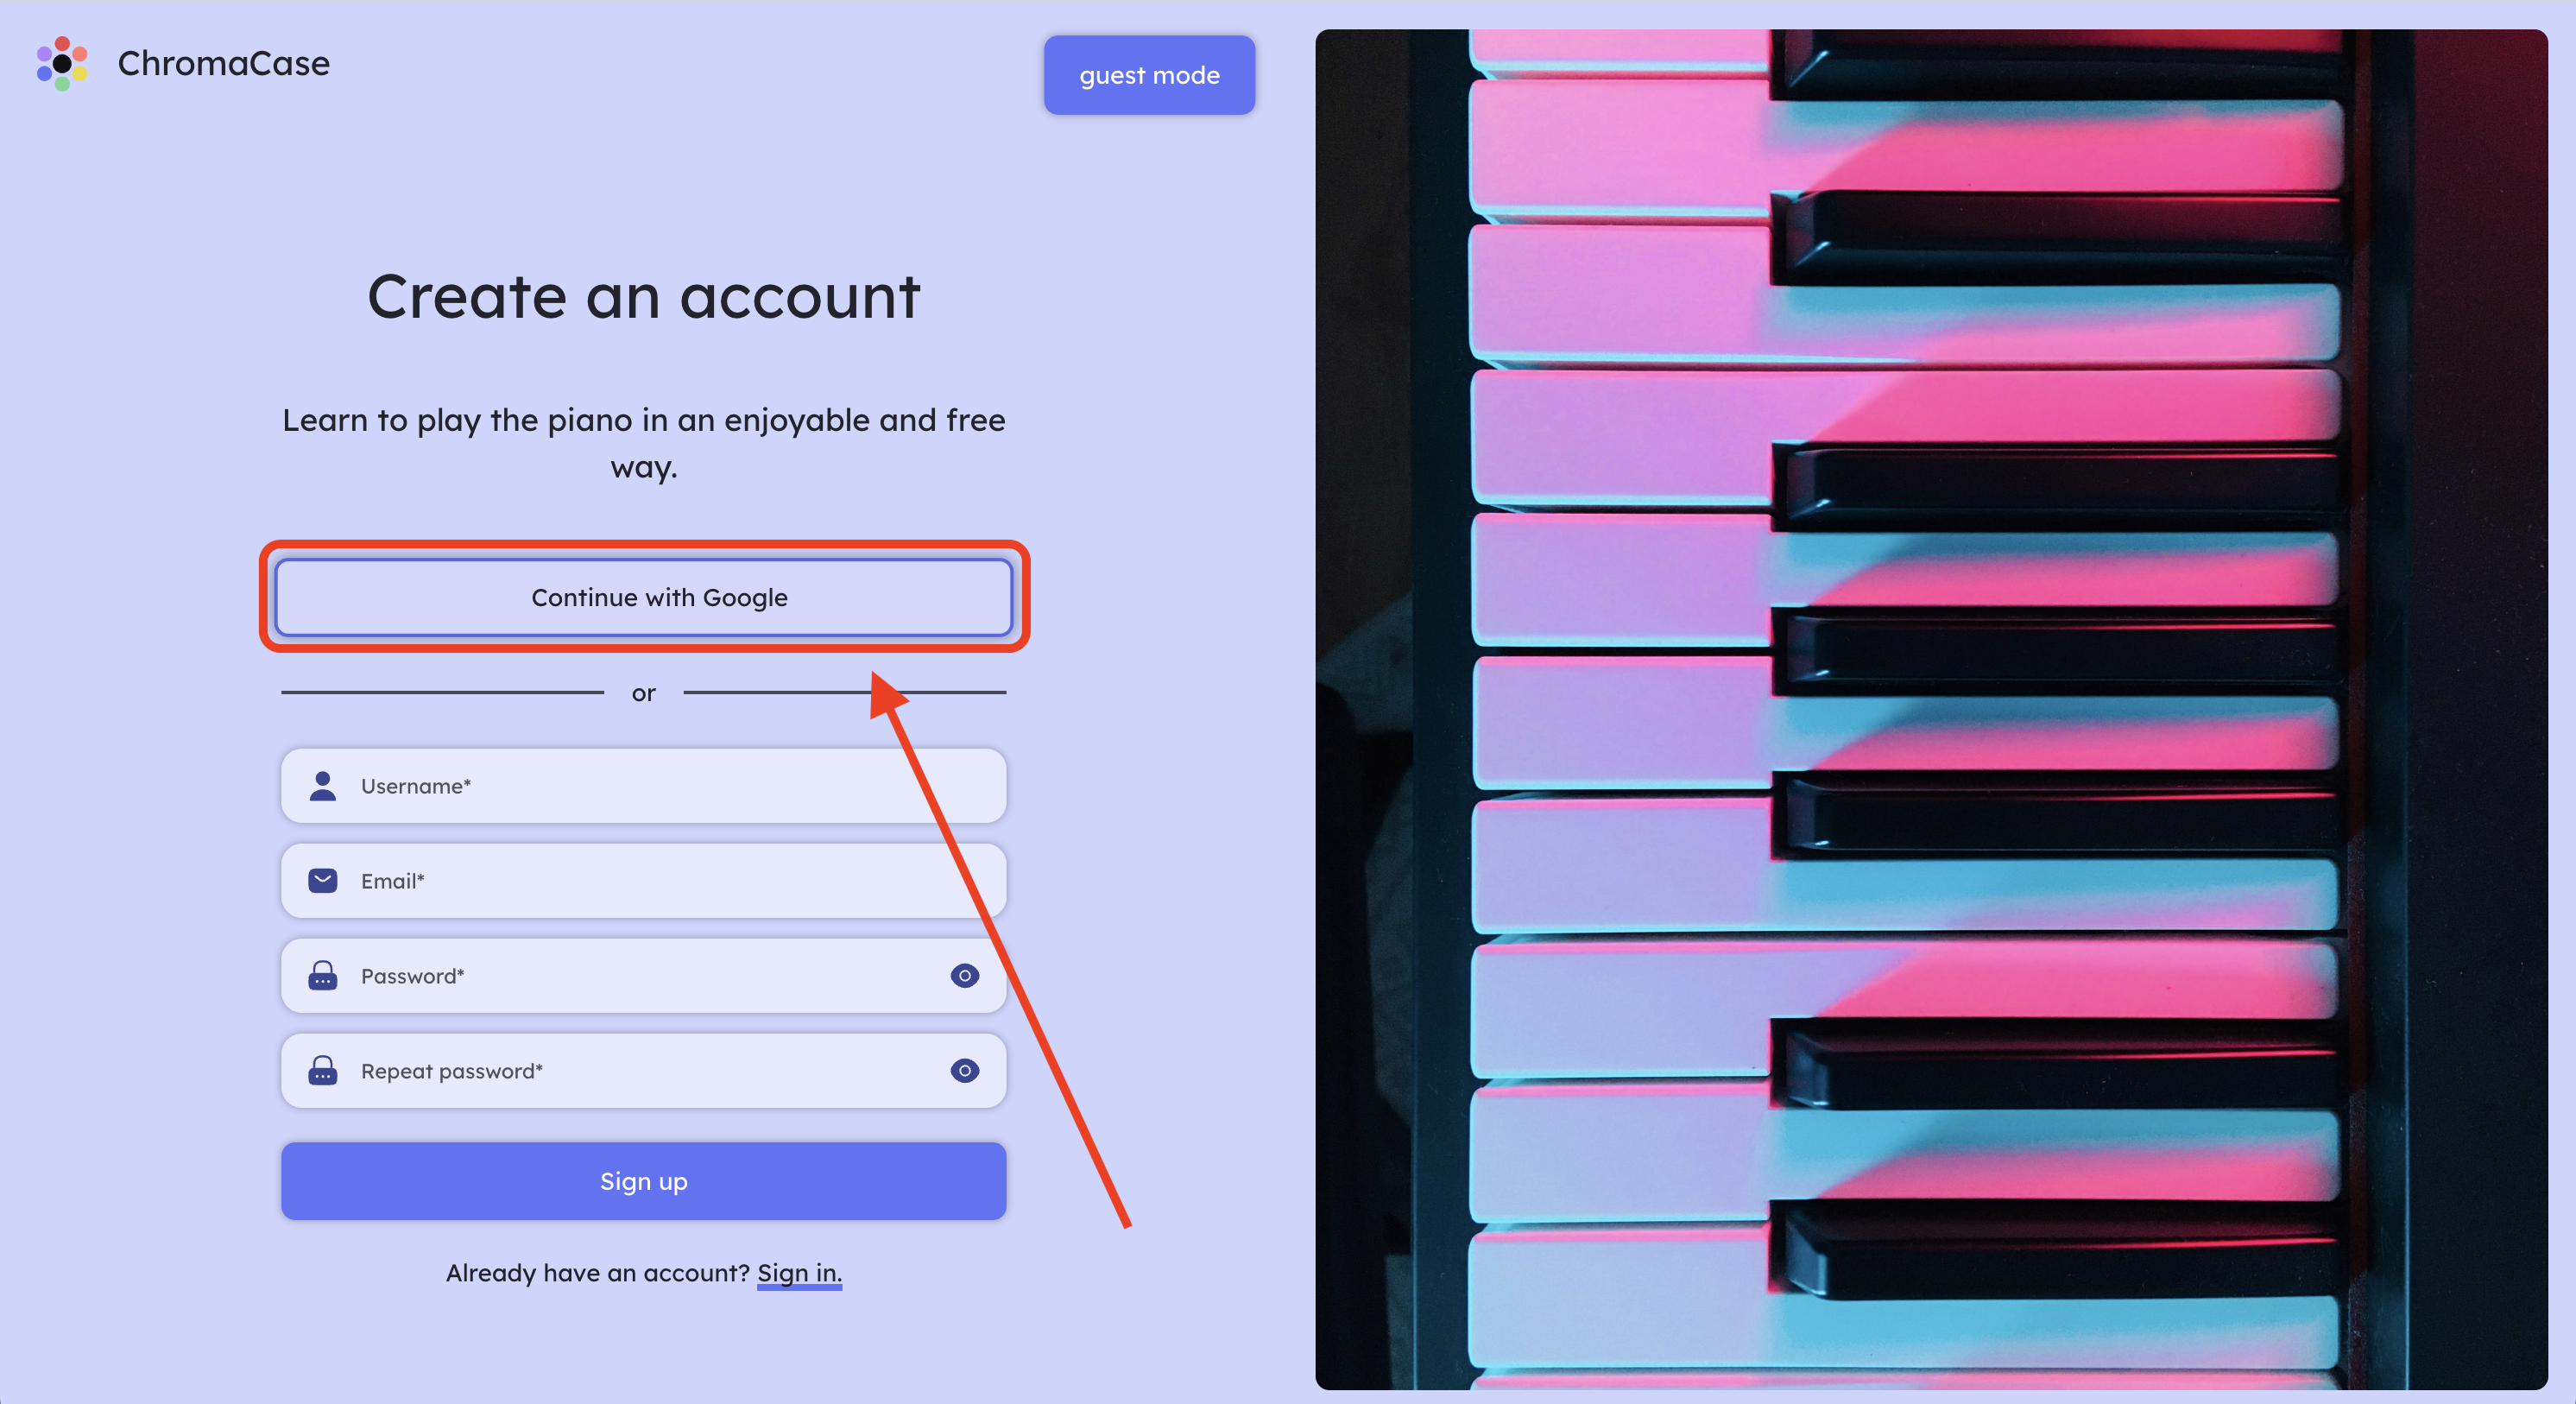
\includegraphics[width=\linewidth]{../\dir/guide/auth/register-google.png}
	\end{center}
	\caption{Créer un compte avec Google}
	\label{fig:signup-google}
\end{figure}